\label{propuesta}
Una vez introducida la teoría de conjuntos difusos en el capítulo previo y de dar una introducción a las bases de datos no relacionales, vamos a realizar una propuesta para la base de datos NoSQL, MongoDB, para dotarla de capacidad para la el manejo de datos difusos.

En la literatura podemos encontrar trabajos con propuestas para bases de datos NoSQL, véase \cite{fuzzyquerygraph, fuzzyquerygraph2, fuzzyquerygraph3}, donde se pueden encontrar propuestas para bases de datos basadas en grafos o \cite{fuzzyqueryhbase} donde se habla de modelado de conjuntos difusos en la base de datos HBase. En \cite{fuzzyquerymongo} podemos encontrar una propuesta para realizar consultas difusas en la base de datos MongoDB, el cuál hemos utilizado para sacar algunas ideas sobre las que se basan nuestra propuesta.

El objetivo de la propuesta que se presenta en este trabajo es mantener la compatibilidad con el funcionamiento estándar de MongoDB, mediante el uso del lenguaje proporcionado y de los mecanismos para representar datos que éste proporciona, para representar los tipos de datos difusos considerados e implementar los mecanismos para la elaboración de las consultas difusas sobre los mismos.

\section{Representación de información en MongoDB}

Dependiendo del tipo de dato, acordamos su representación como sigue:

\begin{itemize}
    \item Datos precisos: Hacen referencia a los datos comunes de MongoDB, enteros, fechas, cadenas de texto, arrays, documentos... Estos datos se seguirán representando con el tipo de dato correspondiente y se trabajará con ellos de forma nativa.
    \item Datos difusos: Como ya adelantamos en los capítulos previos, la forma de trabajar con datos difusos que hemos utilizado es mediante los números difusos \ref{fuzzynumbers} de tipo \textbf{trapezoides} \ref{trapezoidrepresentation}. Para representar esto en MongoDB hemos utilizado \texttt{arrays} con cuatro elementos de tipo numérico.
\end{itemize}

\begin{example}
Vamos a introducir una colección que nos valdrá de ejemplo a lo largo del capítulo para afianzar los conceptos y hacer las demostraciones de las implementaciones que se irán viendo.

El problema que nos planteamos es una base de datos con viviendas. La motivación de este tipo de datos es que algunos de los atributos que utiliza, pueden tratarse fácilmente como difusos, por ejemplo, cuando hablamos del precio o de la superficie de una vivienda, habitualmente en el lenguaje oral es fácil definirlo con un rango de valores o una expresión imprecisa: ``...quiero gastarme entre $110000$€ y $120000$€...'', ``...me gustaría una casa que tenga alrededor de $100m^2$...''.

Un ejemplo de un documento de esta colección quedaría:

\begin{lstlisting}[numbers=none]
{
    _id: ObjectId("5b2501805d492f2c6f51a79e"),
    id_inm: 318.0,
    tipo: "PISO",
    precio: [116625.0, 129218.0, 131771.0, 137828.0],
    habitaciones: [2.0, 2.0, 3.0, 3.0],
    superficie: [60.0, 60.0, 60.0, 60.0],
    descripcion: "* CHURRIANA DE LA VEGA, 60 m2 utiles, 2 habitaciones, 1 bano, cocina amueblada, salon, suelos marmol, ascensor, puerta blindada, climalit, exterior, garaje. Ano 2005. Oportunidad!!! Precio: 129.217,60 euros (21.500.000 pts) Ref. 00232 Inm. Aqaba Tlf. 958 26 53 63 / 669 45 41 76."
}
\end{lstlisting}

donde los campos \texttt{precio},  \texttt{superficie} y \texttt{habitaciones} son campos difusos. Nótese, que para que el campo siempre se represente como un trapezoide de cuatro posiciones, hemos utilizado la notación descrita en \ref{notaciontrapezoide}.
\end{example}

\section{Fuzzy Find}

En \cite{tesismedina} se expuso un módulo para permitir extender la capacidad de un SGBDR clásico para que pueda representar y manipular información imprecisa. En este trabajo se ha realizado una prueba de concepto sobre MongoDB mediante la implementación del comando \textbf{fuzzy\_find}, que nos permitirá realizar consultas sobre una base de datos que contenga datos de tipo difuso.

Para llevar a cabo esto, la utilidad que nos provee MongoDB para \href{https://docs.mongodb.com/manual/tutorial/store-javascript-function-on-server/}{almacenar funciones javascript en el servidor de MongoDB}, nos permite su uso en cualquier contexto javascript.

Consideramos una primera alternativa de implementación para esa función basada en el uso del operador de agregación \texttt{map-reduce} descrito en \ref{mapreduce}, pero tras unas pruebas con una cantidad de datos relativamente grande, no obteníamos el rendimiento que esperábamos, las consultas eran demasiado lentas y descartamos esta opción en favor de utilizar el operador de agregación \texttt{pipeline}, véase la sección \ref{pipeline}. Este operador proporciona más opciones de utilidad para nuestro propósito, nos permite utilizar índices y nos ofrece un rendimiento muy superior a la opción basada en el uso de \texttt{map-reduce}.

\texttt{Fuzzy\_find} es un comando de consulta generalizado, en el sentido de que permite expresar consultas clásicas, véase ejemplo~\ref{example:viviendasqueries}, sin cláusulas difusas, y consultas que combinen cláusulas clásicas con cláusulas difusas. De este modo no solo no pierde la funcionalidad de la que mongo provee inicialmente sino que la extiende.

\subsection{Sintaxis del comando \texttt{fuzzy\_find}}

La cabecera de la función \texttt{fuzzy\_find} es la siguiente:

\begin{verbatim}
fuzzy_find(collection, filter, projection, count_name=null)
\end{verbatim}
%
donde los parámetros son:

\begin{itemize}
    \item \textbf{collection}: Nombre de la colección sobre la que se va a ejecutar la consulta.
    \item \textbf{filter}: JSON con la consulta que se va a realizar. Utiliza el formato estándar de MongoDB para especificar las condiciones sobre los documentos a recuperar, incluyendo todos los operadores estándar junto con los operadores que introducimos en nuestra propuesta destinados a expresar condiciones de consulta difusas. Estos operadores los describiremos en la próxima sección.
    \item \textbf{projection}: JSON para la etapa de proyección. Además de usan el formato estándar de MongoDB incorpora operadores específicos para la visualización de datos difusos.
    \item \textbf{count\_name}: Campo opcional. Si se especifica una cadena de texto se añade la etapa \textit{count}\footnote{\url{https://docs.mongodb.com/manual/reference/operator/aggregation/count/}} para devolver la cantidad de documentos recuperados en lugar de los propios documentos.
\end{itemize}

Veamos la sintaxis propuesta mediante un ejemplo.

\begin{example}\label{example:viviendasqueries}

Supongamos una colección \texttt{viviendas} conteniendo los siguientes documentos:

\begin{lstlisting}[numbers=none]
{
    _id: ObjectId("5b2501805d492f2c6f51a79e"),
    id_inm: 318.0,
    tipo: "PISO",
    precio: [116625.0,129218.0,131771.0,137828.0],
    habitaciones: [2.0,2.0,3.0,3.0],
    superficie: [60.0,60.0,60.0,60.0],
    descripcion: "* CHURRIANA DE LA VEGA, 60 m2 utiles, 2 habitaciones, 1 bano, cocina amueblada, salon, suelos marmol, ascensor, puerta blindada, climalit, exterior, garaje. Ano 2005. Oportunidad!!! Precio: 129.217,60 euros (21.500.000 pts) Ref. 00232 Inm. Aqaba Tlf. 958 26 53 63 / 669 45 41 76."
}
{
    _id: ObjectId("5b2501805d492f2c6f51a79f"),
    id_inm: 319.0,
    tipo: "PAREADO",
    precio: [131760.0,132000.0,136674.0,139381.0],
    habitaciones: [2.0,2.0,3.0,3.0],
    superficie: [75.0,75.0,75.0,75.0],
    descripcion: "* CHURRIANA DE LA VEGA, 75 m2. 2 dormitorios, bano, cocina y salon. Plaza de garaje. Nuevo a estrenar. Buenas calidades. Precio 132.000 euros. Inm. Alhamar Tlf. 958 26 68 90."
}
{
    _id: ObjectId("5b2501805d492f2c6f51a7a0"),
    id_inm: 321.0,
    tipo: "PISO",
    precio: [136568.0,138000.0,138900.0,139268.0],
    habitaciones: [2.0,2.0,3.0,3.0],
    superficie: [78.0,78.0,78.0,78.0],
    descripcion: "* CHURRIANA DE LA VEGA, C/Habana Piso  en construccion de 78 m2,  2 habitaciones,  1 bano, cocina americana, comedor de 21 m2, terraza 6 m2, ,suelos de tarima flotante, pintura lisa, calefaccion totalmente instalada de calor azul.  garaje y trastero, En Construccion, le queda menos de 1 ano. Precio: 138.000,00 euros (22.962.952 pts) Ref:  40323. Inm. Tres Plazas Tlf. 958 25 06 46 / 677 40 97 28."
}
\end{lstlisting}
%
si queremos obtener los documentos que cumplen que el campo \texttt{tipo} es igual a \texttt{``PISO"}, podríamos usar la función \texttt{fuzzy\_find} para ejecutar esa consulta como sigue:
%
\begin{verbatim}
fuzzy_find("viviendas", {tipo: "PISO"}, {})
\end{verbatim}
%
obteniendo el siguiente resultado:
%
\begin{lstlisting}[numbers=none]
{
    _id: ObjectId("5b2501805d492f2c6f51a79e"),
    id_inm: 318.0,
    tipo: "PISO",
    precio: [116625.0,129218.0,131771.0,137828.0],
    habitaciones: [2.0,2.0,3.0,3.0],
    superficie: [60.0,60.0,60.0,60.0],
    descripcion: "* CHURRIANA DE LA VEGA, 60 m2 utiles, 2 habitaciones, 1 bano, cocina amueblada, salon, suelos marmol, ascensor, puerta blindada, climalit, exterior, garaje. Ano 2005. Oportunidad!!! Precio: 129.217,60 euros (21.500.000 pts) Ref. 00232 Inm. Aqaba Tlf. 958 26 53 63 / 669 45 41 76."
}
{
    _id: ObjectId("5b2501805d492f2c6f51a7a0"),
    id_inm: 321.0,
    tipo: "PISO",
    precio: [136568.0,138000.0,138900.0,139268.0],
    habitaciones: [2.0,2.0,3.0,3.0],
    superficie: [78.0,78.0,78.0,78.0],
    descripcion: "* CHURRIANA DE LA VEGA, C/Habana Piso  en construccion de 78 m2,  2 habitaciones,  1 bano, cocina americana, comedor de 21 m2, terraza 6 m2, ,suelos de tarima flotante, pintura lisa, calefaccion totalmente instalada de calor azul.  garaje y trastero, En Construccion, le queda menos de 1 ano. Precio: 138.000,00 euros (22.962.952 pts) Ref:  40323. Inm. Tres Plazas Tlf. 958 25 06 46 / 677 40 97 28."
}
\end{lstlisting}
%
si añadimos una proyección a la función:
%
\begin{verbatim}
fuzzy_find("viviendas", {tipo: "PISO"}, {_id:0, id_inm:1})
\end{verbatim}
%
obtendríamos:
%
\begin{lstlisting}[numbers=none]
{id_inm: 318.0}
{id_inm: 321.0}
\end{lstlisting}

\end{example}

\section{Implementación}

En esta sección se va a detallar la implementación de los algoritmos necesarios para implementar el comando $fuzzy\_find$. Se va a hacer referencia a las líneas del código incluido en el apéndice \ref{appendix:code}.

La implementación se ha realizado en lenguaje Javascript, el motivo principal es preparar scripts que son ejecutables directamente con el comando ``mongo'' especificando la conexión con la base de datos y la ruta al script.
%
\begin{verbatim}
    mongo localhost/mydb fuzzy_find.js
\end{verbatim}
%
de esta forma facilitamos la integración del comando al usuario final.

Para optimizar la búsqueda utilizando el comando \texttt{aggregate}, necesitamos hacer primero una etapa \texttt{match} que filtre lo máximo posible, pues recordemos que esta etapa es la única que aprovechará la indexación para optimizar la búsqueda. Es por esto que no podemos aprovechar directamente las fórmulas para obtener el grado de pertenencia de cada tupla \ref{cdeg} y después evaluar con el umbral deseado, ya que esto obligaría a recorrer todos los documentos de la base de datos antes de filtrar y no sería eficiente. 

Vamos a utilizar las técnicas de \textbf{preselección} y \textbf{selección} basadas en las estudiadas en \cite{indexingstrategies}. La técnica de preselección consiste en calcular los cortes superior, \texttt{U\_CT}, e inferior, \texttt{L\_CT}, sobre el trapezoide que se pretende comparar con los de la base de datos, para calcular estos cortes, es necesario el umbral mínimo (grado de pertenencia) que se quiere considerar, veremos como calcular cada uno de ellos dependiendo del operador en cuestión en las secciones posteriores. La técnica de selección, consistirá en evaluar y comparar los mismos cortes calculados sobre los trapezoides restante y comparar directamente con los cortes obtenidos en la etapa de preselección. Véase la figura~\ref{fig:preselection} obtenida de \cite{indexingstrategies} que ilustra cómo funcionan ambas etapas.

\begin{figure}[h]
  \centering
  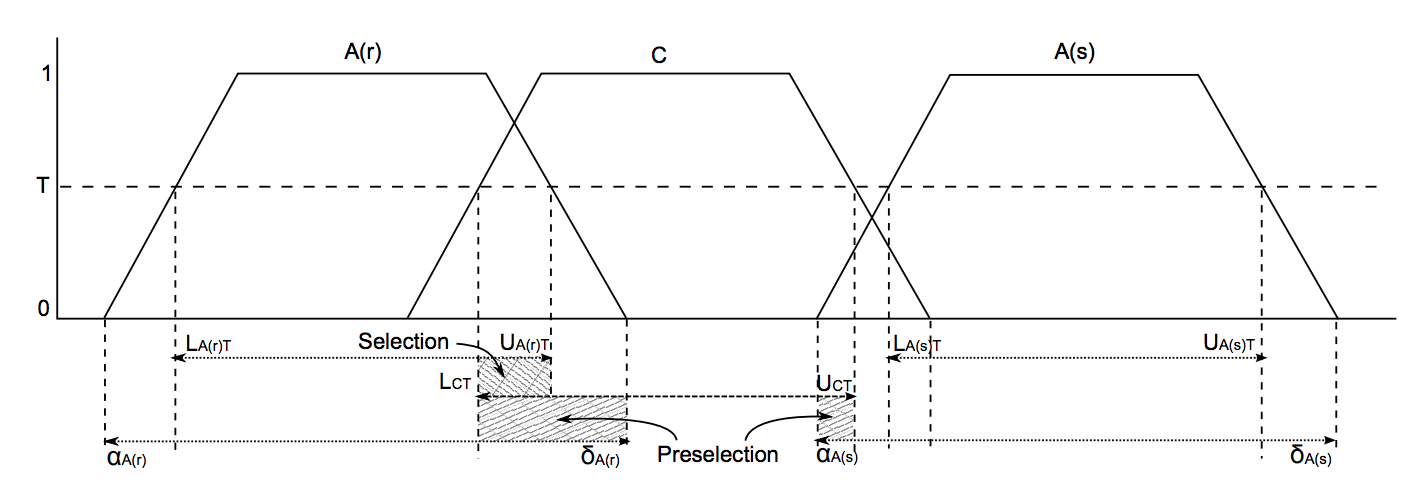
\includegraphics[width=0.9\textwidth]{gfx/preselection.png}
  \caption{\label{fig:preselection}Ejemplo de preselección y selección.}
\end{figure}

\subsection{Implementación de operadores difusos}

Para poder trabajar con cláusulas difusas, se han realizado extensiones de los operados descritos en \ref{mongooperators} para las medidas de posibilidad y necesidad.

Los operadores difusos son operadores ternarios que reciben los siguientes parámetros:

\begin{itemize}
    \item \textbf{field\_name}: Nombre del campo a evaluar. El campo tiene que corresponder con un atributo difuso cuyo valor debe ser un array de cuatro posiciones. 
    \item \textbf{value}: Trapezoide de referencia que estamos comparando.
    \item \textbf{threshold}: Grado mínimo pertenencia que debe cumplir el trapezoide a evaluar para superar el mínimo pedido.
\end{itemize}

Para la etapa de preselección debemos de calcular los cortes inferior y superior, L\_CT y U\_CT, respectivamente con respecto al trapezoide de referencia (el que se pretende comparar con los de la base de datos) y dar ciertas condiciones que deben de verificar alguno de los valores del array de la base de datos con respecto a estos cortes. La etapa de selección consiste en comparar los cortes calculados previamente con los cortes calculados sobre cada uno de los trapezoides almacenados en la base de datos. 

Sean $A$ y $B$ dos distribuciones de posibilidad trapezoidales definidas sobre un dominio ordenado $\Omega$, con $A = \trapezoidA$ y $B=\trapezoidB$ y $T \in [0,1]$ el parámetro \textit{threshold}. Vamos a definir los distintos operadores difusos dependiende del tipo de medida para posibilidad y necesidad.

\subsection{Operador THOLD}

El operador \texttt{\$thold} es un operador que aceptaremos como parámetro extra para todos los operadores difusos, será opcional y en caso de especificarse deberá contener un número entre $0$ y $1$. Será el grado de pertenencia mínimo que esperamos para el valor especificado. Si no se especifica, se tomará por defecto el valor $0$.

\subsection{Operador FEQ}

El operador \texttt{\$feq(A,T)} filtra los documentos $B$ que son \textit{posiblemente} iguales que $A$ para el umbral $T$.

Se calculan los cortes inferior y superior para el trapezoide $A$ \cite{indexingstrategies}:
%
\begin{align*}
    L_{CT} &= T * \beta_A + (1-T)\alpha_A \\
    U_{CT} &= T * \gamma_A + (1-T)\delta_A \\
\end{align*}
%
La etapa de preselección se calcula evaluando:
%
\begin{align*}
    \alpha_B &\leq U_{CT} \\
    \delta_B &\geq L_{CT} \\
\end{align*}
%
Y los elementos seleccionados finalmente son los que cumplan:
%
\begin{align*}
    L_B &\leq U_{CT} \\
    U_B &\geq L_{CT} \\
\end{align*}
%
donde $L_B$ y $U_B$ son los cortes inferior y superior respectivamente para cada documento de la base de datos calculados con las mismas ecuaciones que han calculado $U_{CT}$ y $L_{CT}$ pero con los valores de $B$.
La implementación de este operador puede verse en el apéndice \ref{appendix:code} entre las líneas \ref{code:feq:start} y \ref{code:feq:end}.

\begin{example}
Veamos un ejemplo de una consulta utilizando el operador \texttt{\$feq}:
%
\begin{verbatim}
{"superficie": {"$feq": [80,90,110,120]}}
\end{verbatim}
%
Especificando un umbral mínimo de 0.6:
%
\begin{verbatim}         
{"superficie": {"$feq": [80,90,110,120], "$thold": 0.6}}
\end{verbatim}

\end{example}

\subsection{Operador NFEQ}

El operador \texttt{\$nfeq(A,T)} filtra los documentos $B$ que son \textit{necesariamente} iguales que $A$ para el umbral $T$.

Se calculan los cortes inferior y superior para el trapezoide $A$ \cite{indexingneccesary}:
%
\begin{align*}
    L_{CT} &= T * \beta_A + (1-T)\alpha_A \\
    U_{CT} &= T * \gamma_A + (1-T)\delta_A \\
\end{align*}
%
La etapa de preselección se calcula evaluando:
%
\begin{align*}
    \beta_B &\geq L_{CT} \\
    \gamma_B &\leq U_{CT} \\
\end{align*}
%
Y los elementos seleccionados finalmente son los que cumplan:
%
\begin{align*}
    U_B &\leq U_{CT} \\
    L_B &\geq L_{CT} \\
\end{align*}
%
donde $L_B$ y $U_B$ son los cortes inferior y superior respectivamente para cada documento de la base de datos dado por:
%
\begin{align*}
    L_B &= T * \alpha_B + (1-T)\beta_B \\
    U_B &= T * \delta_B + (1-T)\gamma_B \\
\end{align*}
%
La implementación de este operador puede verse en el apéndice \ref{appendix:code} entre las líneas \ref{code:nfeq:start} y \ref{code:nfeq:end}.

\begin{example}
Veamos un ejemplo de una consulta utilizando el operador \texttt{\$nfeq}:
%
\begin{verbatim}
{"superficie": {"$nfeq": [80,90,110,120]}}
\end{verbatim}
%
Especificando un umbral mínimo de 0.4:
%
\begin{verbatim}         
{"superficie": {"$nfeq": [80,90,110,120], "$thold": 0.4}}
\end{verbatim}

\end{example}

\subsection{Operador FGT}

El operador \texttt{\$fgt(A,T)} filtra los documentos $B$ que son \textit{posiblemente} mayores que $A$ para el umbral $T$.

En este caso, no hay corte superior, por lo que solo calculamos el inferior:
%
\begin{align*}
    L_{CT} &= T * \delta_A + (1-T)\gamma_A \\
\end{align*}
%
La etapa de preselección se calcula evaluando:
%
\begin{align*}
    \delta_B \geq L_{CT}
\end{align*}
%
Y los elementos seleccionados finalmente son los que cumplan:
%
\begin{align*}
    L_B \geq L_{CT} \\
\end{align*}
%
donde $L_B$ es el corte inferior para cada documento de la base de datos dado por:
%
\begin{align*}
    L_B &= T * \gamma_B + (1-T)\delta_B
\end{align*}
%
La implementación de este operador puede verse en el apéndice \ref{appendix:code} entre las líneas \ref{code:fgt:start} y \ref{code:fgt:end}.

\begin{example}
Veamos un ejemplo de una consulta utilizando el operador \texttt{\$fgt}:
%
\begin{verbatim}
{"superficie": {"$fgt": [80,90,110,120]}}
\end{verbatim}

\end{example}

\subsection{Operador NFGT}

El operador \texttt{\$nfgt(A,T)} filtra los documentos $B$ que son \textit{necesariamente} mayores que $A$ para el umbral $T$.

En este caso, no hay corte superior, por lo que solo calculamos el inferior:
%
\begin{align*}
    L_{CT} &= T * \delta_A + (1-T)\gamma_A \\
\end{align*}
%
La etapa de preselección se calcula evaluando:
%
\begin{align*}
    \beta_B \geq L_{CT}
\end{align*}
%
Y los elementos seleccionados finalmente son los que cumplan:
%
\begin{align*}
    L_B \geq L_{CT} \\
\end{align*}
%
donde $L_B$ es el corte inferior para cada documento de la base de datos dado por:
%
\begin{align*}
    L_B &= T * \alpha_B + (1-T)\beta_B
\end{align*}
%
La implementación de este operador puede verse en el apéndice \ref{appendix:code} entre las líneas \ref{code:nfgt:start} y \ref{code:nfgt:end}.

\begin{example}
Veamos un ejemplo de una consulta utilizando el operador \texttt{\$nfgt}:
%
\begin{verbatim}
{"superficie": {"$nfgt": [80,90,110,120]}}
\end{verbatim}

\end{example}

\subsection{Operador FGTE}

El operador \texttt{\$fgte(A,T)} filtra los documentos $B$ que son \textit{posiblemente} mayores o iguales que $A$ para el umbral $T$.

En este caso, no hay corte superior, por lo que solo calculamos el inferior:
%
\begin{align*}
    L_{CT} &= T * \beta_A + (1-T)\alpha_A \\
\end{align*}
%
La etapa de preselección se calcula evaluando:
%
\begin{align*}
    \delta_B \geq L_{CT}
\end{align*}
%
Y los elementos seleccionados finalmente son los que cumplan:
%
\begin{align*}
    L_B \geq L_{CT} \\
\end{align*}
%
donde $L_B$ es el corte inferior para cada documento de la base de datos dado por:
%
\begin{align*}
    L_B &= T * \gamma_B + (1-T)\delta_B
\end{align*}
%
La implementación de este operador puede verse en el apéndice \ref{appendix:code} entre las líneas \ref{code:fgte:start} y \ref{code:fgte:end}.

\begin{example}
Veamos un ejemplo de una consulta utilizando el operador \texttt{\$fgte}:
%
\begin{verbatim}
{"superficie": {"$fgte": [80,90,110,120]}}
\end{verbatim}

\end{example}

\subsection{Operador NFGTE}

El operador \texttt{\$nfgte(A,T)} filtra los documentos $B$ que son \textit{necesariamente} mayores o iguales que $A$ para el umbral $T$.

En este caso, no hay corte superior, por lo que solo calculamos el inferior:
%
\begin{align*}
    L_{CT} &= T * \beta_A + (1-T)\alpha_A \\
\end{align*}
%
La etapa de preselección se calcula evaluando:
%
\begin{align*}
    \beta_B \geq L_{CT}
\end{align*}
%
Y los elementos seleccionados finalmente son los que cumplan:
%
\begin{align*}
    L_B \geq L_{CT} \\
\end{align*}
%
donde $L_B$ es el corte inferior para cada documento de la base de datos dado por:
%
\begin{align*}
    L_B &= T * \alpha_B + (1-T)\beta_B
\end{align*}
%
La implementación de este operador puede verse en el apéndice \ref{appendix:code} entre las líneas \ref{code:nfgte:start} y \ref{code:nfgte:end}.

\begin{example}
Veamos un ejemplo de una consulta utilizando el operador \texttt{\$nfgte}:
%
\begin{verbatim}
{"superficie": {"$nfgte": [80,90,110,120]}}
\end{verbatim}

\end{example}

\subsection{Operador FLT}

El operador \texttt{\$flt(A,T)} filtra los documentos $B$ que son \textit{posiblemente} menores que $A$ para el umbral $T$.

En este caso, no hay corte inferior, por lo que solo calculamos el superior:
%
\begin{align*}
    U_{CT} &= T * \alpha_A + (1-T)\beta_A \\
\end{align*}
%
La etapa de preselección se calcula evaluando:
%
\begin{align*}
    \alpha_B \leq U_{CT}
\end{align*}
%
Y los elementos seleccionados finalmente son los que cumplan:
%
\begin{align*}
    U_B \leq U_{CT} \\
\end{align*}
%
donde $U_B$ es el corte inferior para cada documento de la base de datos dado por:
%
\begin{align*}
    U_B &= T * \beta_B + (1-T)\alpha_B
\end{align*}
%
La implementación de este operador puede verse en el apéndice \ref{appendix:code} entre las líneas \ref{code:flt:start} y \ref{code:flt:end}.

\begin{example}
Veamos un ejemplo de una consulta utilizando el operador \texttt{\$flt}:
%
\begin{verbatim}
{"superficie": {"$flt": [80,90,110,120]}}
\end{verbatim}

\end{example}

\subsection{Operador NFLT}

El operador \texttt{\$nflt(A,T)} filtra los documentos $B$ que son \textit{necesariamente} menores que $A$ para el umbral $T$.

En este caso, no hay corte inferior, por lo que solo calculamos el superior:
%
\begin{align*}
    U_{CT} &= T * \alpha_A + (1-T)\beta_A \\
\end{align*}
%
La etapa de preselección se calcula evaluando:
%
\begin{align*}
    \gamma_B \leq U_{CT}
\end{align*}
%
Y los elementos seleccionados finalmente son los que cumplan:
%
\begin{align*}
    U_B \leq U_{CT} \\
\end{align*}
%
donde $U_B$ es el corte inferior para cada documento de la base de datos dado por:
%
\begin{align*}
    U_B &= T * \delta_B + (1-T)\gamma_B
\end{align*}
%
La implementación de este operador puede verse en el apéndice \ref{appendix:code} entre las líneas \ref{code:nflt:start} y \ref{code:nflt:end}.

\begin{example}
Veamos un ejemplo de una consulta utilizando el operador \texttt{\$nflt}:
%
\begin{verbatim}
{"superficie": {"$nflt": [80,90,110,120]}}
\end{verbatim}

\end{example}

\subsection{Operador FLTE}

El operador \texttt{\$flte(A,T)} filtra los documentos $B$ que son \textit{posiblemente} menores o iguales que $A$ para el umbral $T$.

En este caso, no hay corte inferior, por lo que solo calculamos el superior:
%
\begin{align*}
    U_{CT} &= T * \gamma_A + (1-T)\delta_A \\
\end{align*}
%
La etapa de preselección se calcula evaluando:
%
\begin{align*}
    \alpha_B \leq U_{CT}
\end{align*}
%
Y los elementos seleccionados finalmente son los que cumplan:
%
\begin{align*}
    U_B \leq U_{CT} \\
\end{align*}
%
donde $U_B$ es el corte inferior para cada documento de la base de datos dado por:
%
\begin{align*}
    U_B &= T * \beta_B + (1-T)\alpha_B
\end{align*}
%
La implementación de este operador puede verse en el apéndice \ref{appendix:code} entre las líneas \ref{code:flte:start} y \ref{code:flte:end}.

\begin{example}
Veamos un ejemplo de una consulta utilizando el operador \texttt{\$flte}:
%
\begin{verbatim}
{"superficie": {"$flte": [80,90,110,120]}}
\end{verbatim}

\end{example}

\subsection{Operador NFLTE}

El operador \texttt{\$nflte(A,T)} filtra los documentos $B$ que son \textit{necesariamente} menores o iguales que $A$ para el umbral $T$.

En este caso, no hay corte inferior, por lo que solo calculamos el superior:
%
\begin{align*}
    U_{CT} &= T * \gamma_A + (1-T)\delta_A \\
\end{align*}
%
La etapa de preselección se calcula evaluando:
%
\begin{align*}
    \gamma_B \leq U_{CT}
\end{align*}
%
Y los elementos seleccionados finalmente son los que cumplan:
%
\begin{align*}
    U_B \leq U_{CT} \\
\end{align*}
%
donde $U_B$ es el corte inferior para cada documento de la base de datos dado por:
%
\begin{align*}
    U_B &= T * \delta_B + (1-T)\gamma_B
\end{align*}
%
La implementación de este operador puede verse en el apéndice \ref{appendix:code} entre las líneas \ref{code:nflte:start} y \ref{code:nflte:end}.

\begin{example}
Veamos un ejemplo de una consulta utilizando el operador \texttt{\$nflte}:
%
\begin{verbatim}
{"superficie": {"$nflte": [80,90,110,120]}}
\end{verbatim}

\end{example}
